%======================================================================
\chapter{Stable Matching Polytope}
%======================================================================
\paragraph{}
In this we focus on a polyhedral characterization of the set of
incidence vectors of stable matchings.  Vande Vate first provided such
a description in \cite{vate1989linear} for the special case where $G$
is a complete bipartite graph.  Rothblum \cite{rothblum1992characterization} later generalized Vande Vate's result to incomplete preference lists and simplified the proof of integrality via an extreme point argument.
\paragraph{}
We provide a simpler, more compact argument for the integrality of Rothblum's formulation. Our arguments are elementary and rely solely on some well-known results on stable matchings as well as some knowledge of the local structure of extreme points in our formulation to achieve the desired result. This proof operates in the spirit of iterative rounding as discussed in \ref{IR}. We say it is iterative rounding in spirit because, while it does not follow the strict approach of iterative rounding, it proves that there is an integral variable in every extreme point and analyses the result of dropping that variable and applying induction to the smaller problem instance to obtain a contradiction. Since it is an argument by minimal counterexample it is not immediately clear how to extend this proof to an iterative rounding algorithm.
\section{Linear Description}
\paragraph{Notation}
We will use some notation to ease exposition. Suppose $G=(A\cup B, E)$ is a bipartite graph. Let $S \subseteq E$ and let $x \in \R^{\size{E}}$. Then we denote $\sum_{e\in S} x_e$ by $x(S)$. Suppose every vertex in $A \cup B$ has strict preference orders over its neighbours in $G$ as in a stable matching instance. Then for any $a\in A$ and $b \in B$ we let
$$\delta^{>a}(b) = \{a'b \in E(G): a' >_b a\}.$$
We can define $\delta^{>b}(a)$ analogously, and further replace $>$ with $<, \leq, \geq, =$ in the natural way.
\paragraph{Linear Description}
We will begin with a linear description of a polytope which we claim has incidence vectors of stable matchings as its extreme points. This polytope is the matching polytope described in \ref{GT:MWM} with added ``stability" constraints. If we let $G=(A\cup B, E)$ be a bipartite graph with preferences then we will denote the so-called stable matching polytope of $G$ by $P(G)$ and it has the following description:
\begin{align}
x(\delta(v)) &\leq 1, &\text{for all } v \in A\cup B \label{constraint:one}\\
x_e &\geq 0, &\text{for all } e \in E \label{constraint:nonneg}\\
x(\delta^{>a}(b)) + x(\delta^{>b}(a)) + x_{ab} &\geq 1, &\text{for all } ab \in E.\label{constraint:stab}
\end{align}
Our major theorem of this chapter is to demonstrate that $P(G)$ is integral, but first we must verify that indeed the integral extreme points of $P(G)$ are exactly the incidence vectors of stable matchings in $G$.
\begin{lemma}\label{lemma:int-P}
Let $x \in \R^{\size{E}}$. Then $x$ is an integral extreme point of $P(G)$ if and only if there exists a stable matching $M$ of $G$ such that $x = \chi(M)$.
\end{lemma}
\begin{proof}
Suppose that $x$ is an integral extreme point of $P(G)$. By constraints \ref{constraint:one} and \ref{constraint:nonneg}, $x$ is the incidence vector of some matching $M$ of $G$. Suppose that $M$ is not stable, that is to say there exists $ab \in E$ which blocks $M$. But $ab$ satisfies:
$$x(\delta^{>a}(b)) + x(\delta^{>b}(a)) + x_{ab} \geq 1.$$
Since $x$ is integral this implies that either
$$x(\delta^{>a}(b)) = 1 \quad\text{or}\quad  x(\delta^{>b}(a)) = 1 \quad\text{or}\quad x_{ab}=1,$$
and as $ab \not\in M$ we known $\chi(M)_{ab} = x_{ab}=0$. Thus we have two cases:
$$x(\delta^{>a}(b)) = 1 \quad\text{or}\quad  x(\delta^{>b}(a)) = 1.$$
In the first case there exists $ab' \in \delta^{>a}(b)$ for which $x_{ab'} = 1$ and hence $ab' \in M$  with $b' >_a b$. Thus in the first case $ab$ does not block $M$. Similarly in the second case there exists $a' >_b a$ with $a'b \in M$ and hence $ab$ does not block $M$ in either case. Therefore $M$ is stable.
\paragraph{}
Now let $M$ be a stable matching in $G$, and suppose  $x = \chi(M)$. Since $M$ is a matching $x(\delta(v)) \leq 1$ for all $v \in A \cup B$ and $x_e \geq 0$ for all $e \in E$. Hence it remains to verify that $x$ satisfies constraints \ref{constraint:stab}. Indeed let $ab \in E$. If $ab \in M$ then $1 = \chi(M)_{ab} = x_{ab}$ and so \ref{constraint:stab} is satisfied for $ab$. Now if $ab \not\in M$ then, since $M$ is stable, $(a,b)$ is not a blocking pair. So there exists $ab' \in M$ with $b' >_a b$ or there exists $a'b \in M$ with $a' >_b a$. In the former case $x(\delta^{>b}(a)) = 1$ and in the latter $x(\delta^{>a}(b)) = 1$. In either case \ref{constraint:stab} is satisfied for $ab$ as desired.  
\end{proof}
\section{Proof of Integrality}
\paragraph{}
In this section we build the necessary theory towards a proof that $P(G)$ is integral.
\subsection{Edges of Polytopes}
\paragraph{}
Before discussing the proof proper we need to take a slight detour to review some more elementary polyhedral geometry.

\paragraph{}Let $x^1, x^2 \in \R^n$. Then $x \in \R^n$ is a {\it convex combination} of $x^1, x^2$ provided there exists $\lambda \in \R$ with $0 \leq \lambda \leq 1$ and $$x = \lambda x^1 + (1-\lambda)x^2.$$

\paragraph{}Let $P\subseteq \R^n$ be a polytope. Then the hyperplane given by $(h,\delta)$ is said to describe a {\it valid inequality} for $P$ if for all $x \in P$ $h^Tx \leq \delta$.

\paragraph{}Let $P \subseteq \R^n$ be a polytope. For our purposes we define an {\it edge} of $P$ to be a set $F$ of the form $$F = P \cap \{x \in \R^n: h^Tx = \delta \}$$ where $(h,\delta)$ describes a valid inequality for $P$, and there exist $x^1, x^2 \in P$ such that $x^1$ and $x^2$ are vertices of $P$ for which all $x \in F$ are a convex combination of $x^1, x^2$.

\begin{lemma}\label{lemma:edge-midpoint}
Let $P \subseteq \R^n$ be a polytope. Let $F$ be an edge of $P$ defined by valid inequality $(h,\delta)$ and extreme points $x^1, x^2$. Suppose there exist $y^1, y^2 \in \R^n$ neither of which is a convex combination of $x^1, x^2$ satisfying
$$\frac{1}{2}x^1 + \frac{1}{2} x^2 = \frac{1}{2} y^1 + \frac{1}{2}y^2.$$
Then at most one of $y^1, y^2$ lies in $P$.
\end{lemma}
\begin{figure}
\centering
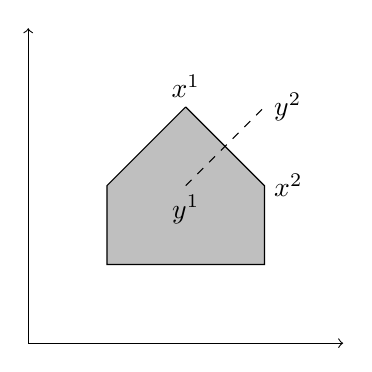
\begin{tikzpicture}
\draw[<->] (1,4) -- (1,0) -- (5,0);

\draw[fill=lightgray] (3,3) node[above]{$x^1$} -- (4,2)node[right]{$x^2$} -- (4,1) -- (2,1) -- (2,2) -- (3,3);

\draw[dashed] (3,2) node[below]{$y^1$} -- (4,3) node[right]{$y^2$};
\end{tikzpicture}
\caption{Visualizing Lemma \ref{lemma:edge-midpoint}}
\small
\begin{flushleft}
The extreme points $x^1$ and $x^2$ define an edge of this polytope. From the visual one can see that any line segment intersecting the edge between $x^1$ and $x^2$ cannot have both its endpoints $y^1$ and $y^2$ in the polytope.
\end{flushleft}
\end{figure}
\begin{proof}
Let $$x = \frac{1}{2}x^1 + \frac{1}{2} x^2 = \frac{1}{2} y^1 + \frac{1}{2}y^2.$$ Suppose for a contradiction that $y^1,y^2 \in P$. Since $y^1, y^2 \not\in F$ as $y_1$ and $y_2$ are not convex combinations of $x_1$ and $x_2$, we have
$$h^Ty^1 < \delta \quad\text{and}\quad h^Ty^2 < \delta. $$
So then,
\begin{align*}
h^Tx &= h^T(\frac{1}{2}y^1 + \frac{1}{2}y^2) \\
&= \frac{1}{2}h^Ty^1 + \frac{1}{2}h^Ty^2 \\
&< \frac{1}{2}\delta + \frac{1}{2}\delta \\
&= \delta.
\end{align*}
That is $h^T x < \delta$. But since $x = \frac{1}{2} x^1 + \frac{1}{2}x^2$, $x$ is a convex combination of $x^1, x^2$ and hence $x \in F$. That is $h^T x = \delta$, contradicting $h^T x < \delta$.
\end{proof}
\paragraph{}
Lemma \ref{lemma:edge-midpoint} says intuitively that line segments intersecting the midpoint of an edge of a polytope have at most one endpoint in $P$.
\subsection{Structural Lemmas}
\paragraph{}
In this section we describe some theory connecting the lattice structure of stable matchings described in \ref{SM:STRUCTURE} and the polytope $P(G)$. Going forward we assume that $E(G) \neq \emptyset$ as otherwise $P(G) = \emptyset$ is vacuously integral. Observe that this assumption implies that $0 \not\in P(G)$ as all constraints \ref{constraint:stab} are violated by $0$.
\begin{lemma}\label{lemma:all-same}
Let $M$ and $M'$ be distinct stable matchings in bipartite graph $G$ with preferences. If $\chi(M)$ and $\chi(M')$ are extreme points of $P(G)$ which define an edge of $P(G)$ then either $sup(M,M') = M$ or $sup(M,M') = M'$.
\end{lemma}
\paragraph{}
Before we begin the proof, we make a quick observation. We observe that $sup(M,M') = M$ if and only if $inf(M,M') = M'$. This follows since $sup(M,M') = M$ if and only if $M(a) \geq_a M'(a)$ for all $a \in A$ and hence $inf(M,M') = M'$.
\begin{proof}
Let $S = sup(M,M')$ and $I = inf(M,M')$. Suppose for a contradiction that $S \neq M$ and $S \neq M'$. That is, by our preceding observation, $S$ and $I$ are distinct stable matchings from $M$ and $M'$. We claim that
\begin{equation} \label{claim:chieq}
\chi(M) + \chi(M') = \chi(S) + \chi(I)
 \end{equation}
To see the claim, let $e \in E(G)$. If $e \in M \cap M'$ then the left hand side of $\ref{claim:chieq}$ is $2$, and further $e \in S \cap I$ and hence the right hand side of $\ref{claim:chieq}$ is $2$. If $e \not\in M \cup M'$ then both the left and right hand side of \ref{claim:chieq} are $0$. If $e \in M \backslash M'$ then either $e \in S$ or $e \in I$. In either case the left and right hand side of \ref{claim:chieq} is $1$, and the same holds for $e \in M' \backslash M$. That is the claim holds.
\paragraph{}
By claim \ref{claim:chieq} we observe two things. First that $\chi(S)$ and $\chi(I)$ are not convex combinations of $\chi(M)$ and $\chi(M')$ since $S$ and $I$ are not equal to either of $M$ or $M'$. Second we observe that $$\frac{1}{2}\chi(M) + \frac{1}{2} \chi(M') = \frac{1}{2} \chi(S) + \frac{1}{2} \chi(I).$$
Therefore we are in a position to invoke Lemma \ref{lemma:edge-midpoint}, concluding that one of $\chi(S), \chi(I) \not\in P(G)$. But this contradicts the Lattice Theorem \ref{theorem:lattice} since $S, I$ are stable matchings in $G$ implies that $\chi(S), \chi(I) \in P$  by Lemma \ref{lemma:int-P}.
\end{proof}
\begin{corollary}\label{cor:edge} (Ratier) \cite{ratier1996stable}:
Let $M$ and $M'$ be distinct stable matchings in bipartite graph $G=(A\cup B, E)$ with preferences. If there exist $a \in A$ and $b \in B$ such that
\begin{equation}\label{cond:nonedge}
M(a) >_a M'(a)  \quad\text{and}\quad M(b) >_b M'(b)
\end{equation}
then $\chi(M)$ and $\chi(M')$ do not define an edge of the polytope $P(G)$.
\end{corollary}
\begin{proof}
Since $M(a) >_a M'(a)$, $aM(a) \in sup(M,M')$. That is $$sup(M,M') \cap M \neq \emptyset$$ and since $M'(a) \neq M(a)$, 
$$sup(M,M') \not\subseteq M'.$$
Since $M(b) >_b M'(b)$, $M'(b)b \in sup(M,M')$. That is $$sup(M,M') \cap M' \neq \emptyset$$ and since $M(b) \neq M'(b)$,
$$sup(M,M') \not\subseteq M.$$
Taken together these observations prove that $sup(M,M')$ is a distinct stable matching from $M$ and $M'$. Thus by Lemma \ref{lemma:all-same}, $\chi(M)$ and $\chi(M')$ do not define an edge of $P(G)$.  
\end{proof}
\subsection{Integrality of $P(G)$}
\paragraph{}
We are now ready to provide our proof that $P(G)$ is integral. The strategy is to first show that every extreme point $x$ has some variable $e \in E$ with $x_e \in \{0,1\}$, then, in a minimal counterexample, remove that variable and look at the reduced problem in the smaller variable set. By induction the vertices of the smaller polytope are integral. We will consider a particular edge of this polytope and obtain a contradiction via our structural lemmas of the previous section showing its end vertices cannot define an edge. The details will be made clear as we proceed.
\begin{lemma}\label{lemma:01}
Let $G = (A\cup B, E)$ be a bipartite graph with preferences. Let $x$ be an extreme point of $P(G)$. Then there exists $e \in E(G)$ such that $x_e \in \{0,1\}$.
\end{lemma}
\begin{proof}
By constraints \ref{constraint:nonneg} and \ref{constraint:one} we have that $0 \leq x_e \leq 1$. Suppose for a contradiction that for all $e \in E(G)$, $0 <x_e < 1$. Since $x$ is an extreme point of $P(G)$ with $x>0$ we may invoke Lemma \ref{lemma:rank}, which says that $x$ is defined by $\size{E}$ linearly independent constraints which are tight (satisfied with equality) at $x$ and no such constraints are from constraints \ref{constraint:nonneg}. Thus all such constraints are from \ref{constraint:one} and \ref{constraint:stab}. Let $V_x \subseteq V(G)$ and $E_x \subseteq E(G)$ be such that $V_x$ and $E_x$ respectively contain vertices and edges corresponding to a set of $\size{E}$ linearly independent constraints tight at $x$. That is $V_x$ contains vertices corresponding to constraints from \ref{constraint:one}, $E_x$ contains edges corresponding to constraints from \ref{constraint:stab}, $\size{E} = \size{E_x} + \size{V_x}$, and $$\{\chi(\delta(v)) : v \in V_x\} \cup \{\chi(\delta^{>a}(b)) + \chi(\delta^{>b}(a)) + \chi(\{ab\}): ab \in E_x\}$$ is linearly independent. Choose $V_x$ and $E_x$ in such a way that $\size{V_x}$ is maximized.
\paragraph{}
First observe that $V_x \subsetneq V$. To see this, suppose that $V_x = V$. Then since $G$ is bipartite
$$\sum_{a \in A} \chi(\delta(a)) = \sum_{b \in B} \chi(\delta(b))$$
and hence $\{\chi(\delta(v)) : v \in V=V_x\}$ is not linearly independent. Thus our observation that $V_x \subsetneq V$ holds.
\paragraph{}
For any $v \in V(G)$ denote by $N(v)$ the set $\{ w \in V(G): vw \in \delta(v)\}$ and let $N_{max}(v) \in N(v)$ be such that $N_{max}(v) \geq_v w$ for all $w \in N(v)$. Similarly let $N_{min}(v) \in N(v)$ be such that $N_{min}(v) \leq_v w$ for all $w \in N(v)$.
\paragraph{}
Let $v \in V(G)$. We claim that if $w = N_{max}(v)$ then $vw \not\in E_x$. Indeed suppose for a contradiction that $vw \in E_x$. Since $w = N_{max}(v)$, $\delta^{>w}(v) = \emptyset$ and hence
$$1 \leq x(\delta^{>w}(v)) + x(\delta^{>v}(w)) + x_{vw}  = x(\delta^{\geq v}(w)) \leq x(\delta(w)) \leq 1,$$
shows that $1 = x(\delta^{\geq v}(w))$ and thus $x(\delta^{<v}(w))= 0$. Since $x_e > 0$ for all $e \in E(G)$ this implies that $\delta^{<v}(w)) = \emptyset$. Therefore
$$\chi(\delta(w)) = \chi(\delta^{\geq v}(w)) = \chi(\delta^{>w}(v)) + \chi(\delta^{>v}(w)) + \chi(\{vw\})$$
and hence by linear independence we cannot have both $vw \in E_x$ and $w \in V_x$. Since $vw \in E_x$ this implies $w \not\in V_x$. But then the sets $V_x \cup\{w\}$ and $E_x \backslash\{vw\}$ describe the same vectors as $V_x, E_x$ but $\size{V_x \cup\{w\}} > \size{V_x}$ contradicting our choice of $V_x$. Thus $vw \not\in E_x$. Therefore for any $v \in V(G)$, $vN_{max}(v) \not\in E_x$.
\paragraph{}
Let $v \in V_x$. Let $w = N_{min}(v)$. We claim analogously to the previous claim that $vw \not\in E_x$. Indeed suppose for a contradiction that $vw  \in E_x$. Since $v \in V_x$, by tightness,
$$x(\delta(v)) = 1$$
and since $vw \in E_x$, by tightness,
$$x(\delta^{>v}(w)) + x(\delta^{>w}(v)) + x_{vw} = 1.$$
Since $w = N_{min}(v)$, $\delta^{>w}(v) \cup \{vw\} = \delta(v)$ and hence
$$x(\delta^{>w}(v)) + x_{vw} = x(\delta(v))$$
and
$$\chi(\delta^{>w}(v)) + \chi(\{vw\}) = \chi(\delta(v)).$$
Thus
$$1 = x(\delta^{>v}(w)) + x(\delta^{>w}(v)) + x_{vw} = x(\delta^{>v}(w)) + x(\delta(v)) = x(\delta^{>v}(w)) + 1,$$
which implies that $x(\delta^{>v}(w)) = 0$. Again since $x_e > 0$ for all $e \in E(G)$, this implies that
$$\chi(\delta^{>v}(w)) = 0.$$
So we have that
$$\chi(\delta(v)) = \chi(\delta^{>w}(v)) + \chi(\{vw\}) = \chi(\delta^{>v}(w)) + \chi(\delta^{>w}(v)) + \chi(\{vw\}),$$
and hence by linear independence we cannot have both $vw \in E_x$ and $v \in V_x$. Since $v \in V_x$ this implies $vw \not\in E_x$, a contradiction.

\paragraph{}
We now apply a token argument to demonstrate that $|E|> |E_x| + |V_x|$, a contradiction. The argument will proceed by assigning each $e \in E$ a token which it will distribute according to a pair of rules to $E_x$ and $V_x$. We will argue that each $e \in E_x$ and $v \in V_x$ receives a token, and that some $e \in E_x$ has at least some token fraction leftover. In demonstrating this we have proven the desired claim.
\paragraph{}
Assign each $ab \in E$ a token. Redistribute the tokens according to the following rules:
\begin{enumerate}
\item if $ab \in E_x$ assign the token to $ab \in E_x$
\item otherwise
\begin{enumerate}
\item if $a \in V_x$ assign $\frac{1}{2}$ a token to $a \in V_x$
\item if $b \in V_x$ assign $\frac{1}{2}$ a token to $b \in V_x$.
\end{enumerate}
\end{enumerate}
First it should be clear that these rules are well-defined since no $ab \in E_x$ gives away more than the one token it receives. Let $ab \in E_x$. Obviously from rule $1$, $ab$ receives one token. Now consider $v \in V_x$. Since $x_e<1$ for all $e$ we know $N_{min}(v) \neq N_{max}(v)$, as otherwise $x(\delta(v)) = x_{vN_{min}(v)} < 1$ which contradicts $v \in V_x$ defining a tight constraint. Further by our previous observations, $vN_{min}(v) \not\in E_x$ and $vN_{max}(v) \not\in E_x$. So when the edges $vN_{min}(v)$ and $vN_{max}(v)$ are applying the rules to distribute their token they each give $\frac{1}{2}$ token to $v$ by rule $2$. So $v$ receives at least one token. To complete the proof we need to find some $e \in E$ which did not give away its whole token. We have previously observed that $V_x \subsetneq V(G)$. So let $v \in V(G)\backslash V_x$. Consider the edge $vN_{max}(v)$. Since $vN_{max}(v) \not\in E_x$ it does not give away its token by rule $1$, and since $v \not\in V_x$ it gives away at most half its token by rule $2$. So the edge $vN_{max}(v)$ has at least $\frac{1}{2}$ a token remaining at the end of redistribution. Therefore $\size{E} > \size{E_x} + \size{V_x}$, contradicting that $\size{E} = \size{E_x} + \size{V_x}$.
\end{proof}
\begin{theorem}
Let $G=(A\cup B, E)$ be a bipartite graph with preferences. Then the polytope $P(G)$ is integral.
\end{theorem}
\begin{proof}
Suppose for a contradiction the theorem does not hold. Let $G=(A\cup B, E)$ be a minimal counterexample in terms of $|E|$. It is clear from case analysis that $|E| > 2$. Let $x$ be a non-integral extreme point of $P(G)$. By Lemma \ref{lemma:01} there exists $ab \in E$ such that $x_{ab} \in \{0,1\}$.
\paragraph{}
First we consider the case where $x_{ab} = 0$. Let $P' = P(G) \cap \{x \in \R^{\size{E(G)}} : x_{ab} = 0 \}$. Then $x$ is an extreme point of polytope $P'$ since $P' \subseteq P(G)$. Let $G'$ be the graph with $V(G') = V(G)$ and $E(G') = E(G) \backslash \{ab\}$. Observe that by dropping edge $ab$ $P(G')$ differs from $P(G)$ only in not having constraint \ref{constraint:stab} for $ab$ and constraints \ref{constraint:one} for $a$ and $b$ not counting edge $ab$ (which is equivalent to assigning $x_{ab} = 0$ always), hence we have
$$P' = P(G') \cap \{x \in \R^{\size{E(G')}} : x(\delta^{>a}(b)) + x(\delta^{>b}(a)) \geq 1 \}.$$
Let $H$ be the hyperplane $\{x \in \R^{\size{E(G')}} : x(\delta^{>a}(b)) + x(\delta^{>b}(a)) = 1\}$. Then every extreme point of $P'$ is either an extreme point of $P(G')$ or the intersection of an edge of $P(G')$ with $H$. Since the extreme points of $P(G')$ are integral by our minimality assumption, $x$ must be in the intersection of an edge $F$ of $P(G')$ with $H$. Let $M$ and $M'$ be stable matchings such that $\chi(M)$ and $\chi(M')$ define $F$. Since $x$ is not integral, $x \neq \chi(M)$ and $x \neq \chi(M')$. Also note that neither $\chi(M)$ nor $\chi(M')$ lies on the hyperplane $H$, since $x$ is the unique and distinct intersection of $H$ with the line segment of convex combinations of $\chi(M)$ and $\chi(M')$. Thus from our definition of $H$, since $\chi(M), \chi(M') \not\in H$,  we have $\size{M \cap (\delta^{>a}(b) \cup \delta^{>b}(a))} \neq 1$ and $\size{M' \cap (\delta^{>a}(b) \cup \delta^{>b}(a))} \neq 1$. On the other hand, the line segment of convex combinations of $\chi(M)$ and $\chi(M')$ has a non-empty intersection with $H$, namely $x$,  and so without loss of generality we may assume that $\size{M \cap (\delta^{>a}(b) \cup \delta^{>b}(a))} = 2$ and $\size{M' \cap (\delta^{>a}(b) \cup \delta^{>b}(a))} = 0$ (notice the size of said intersections is at most $2$ by \ref{constraint:one}).
\paragraph{}
Since $\size{M \cap (\delta^{>a}(b) \cup \delta^{>b}(a))} = 2$, $\size{M\cap \delta(a)} \leq 1$ and $\size{M \cap\delta(b)} \leq 1$, we have $M(a) >_a b$ and $M(b) >_b a$. Further since $\size{M' \cap (\delta^{>a}(b) \cup \delta^{>b}(a))} = 0$ we have that $b >_a M'(a)$ and $a >_b M'(b)$. Thus $M(a) >_a M'(a)$ and $M(b) >_b M'(b)$. Critically, this means $M$ and $M'$ satisfy \ref{cond:nonedge} and so by corollary \ref{cor:edge}, $\chi(M)$ and $\chi(M')$ do not define an edge of $P(G')$. This contradicts that they do indeed define an edge of $P(G')$.
\paragraph{}
Finally we consider the case where $x_{ab} = 1$. By constraints \ref{constraint:one} for $a$ and $b$ we see that $x_{e} = 0$ for all $e \in (\delta(a) \cup \delta(b))\backslash \{ab\}$. Thus if there exists $e \in (\delta(a) \cup \delta(b))\backslash \{ab\}$ then $x_e = 0$ and we may run the previous case analysis with edge $e$. So it remains to consider when $(\delta(a) \cup \delta(b))\backslash \{ab\} = \emptyset$. If we let $G'$ be the graph $G$ with edge $ab$ removed then $P(G')$ is described by precisely the same constraints as $P(G)$ with the exclusion of constraint \ref{constraint:stab} for edge $ab$. Let $x'$ be the vector $x$ restricted to variables $E(G)\backslash\{ab\}$. We claim that $x'$ is an extreme point of $P(G')$. By the Rank Lemma \ref{lemma:rank}, $x$ is described by $|E(G)|$ linearly independent tight constraints. Since $\delta(a) = \delta(b) = \{ab\}$, the constraints \ref{constraint:one} for $a$ and $b$ and the constraint \ref{constraint:stab} for $ab$ are pairwise linearly dependent, and in fact equal. Hence at most one of them is in the description of $x$. Thus we can find $|E(G)| -1 = |E(G')|$ linearly independent constraints tight at $x'$ in $P(G')$ by excluding the constraint \ref{constraint:stab} for $ab$ from those which describe $x$. Therefore $x'$ is an extreme point of $P(G')$. So by minimality $x'$ is integral, and thus $x$ is integral.
\end{proof}
\paragraph{}
This theorem is significant because it allows one to be able to solve maximum weight stable matching problems in bipartite graphs in polynomial time via the use of linear programming.